% Options for packages loaded elsewhere
\PassOptionsToPackage{unicode}{hyperref}
\PassOptionsToPackage{hyphens}{url}
%
\documentclass[
]{article}
\usepackage{amsmath,amssymb}
\usepackage{iftex}
\ifPDFTeX
  \usepackage[T1]{fontenc}
  \usepackage[utf8]{inputenc}
  \usepackage{textcomp} % provide euro and other symbols
\else % if luatex or xetex
  \usepackage{unicode-math} % this also loads fontspec
  \defaultfontfeatures{Scale=MatchLowercase}
  \defaultfontfeatures[\rmfamily]{Ligatures=TeX,Scale=1}
\fi
\usepackage{lmodern}
\ifPDFTeX\else
  % xetex/luatex font selection
\fi
% Use upquote if available, for straight quotes in verbatim environments
\IfFileExists{upquote.sty}{\usepackage{upquote}}{}
\IfFileExists{microtype.sty}{% use microtype if available
  \usepackage[]{microtype}
  \UseMicrotypeSet[protrusion]{basicmath} % disable protrusion for tt fonts
}{}
\makeatletter
\@ifundefined{KOMAClassName}{% if non-KOMA class
  \IfFileExists{parskip.sty}{%
    \usepackage{parskip}
  }{% else
    \setlength{\parindent}{0pt}
    \setlength{\parskip}{6pt plus 2pt minus 1pt}}
}{% if KOMA class
  \KOMAoptions{parskip=half}}
\makeatother
\usepackage{xcolor}
\usepackage{longtable,booktabs,array}
\usepackage{calc} % for calculating minipage widths
% Correct order of tables after \paragraph or \subparagraph
\usepackage{etoolbox}
\makeatletter
\patchcmd\longtable{\par}{\if@noskipsec\mbox{}\fi\par}{}{}
\makeatother
% Allow footnotes in longtable head/foot
\IfFileExists{footnotehyper.sty}{\usepackage{footnotehyper}}{\usepackage{footnote}}
\makesavenoteenv{longtable}
\usepackage{graphicx}
\makeatletter
\def\maxwidth{\ifdim\Gin@nat@width>\linewidth\linewidth\else\Gin@nat@width\fi}
\def\maxheight{\ifdim\Gin@nat@height>\textheight\textheight\else\Gin@nat@height\fi}
\makeatother
% Scale images if necessary, so that they will not overflow the page
% margins by default, and it is still possible to overwrite the defaults
% using explicit options in \includegraphics[width, height, ...]{}
\setkeys{Gin}{width=\maxwidth,height=\maxheight,keepaspectratio}
% Set default figure placement to htbp
\makeatletter
\def\fps@figure{htbp}
\makeatother
\setlength{\emergencystretch}{3em} % prevent overfull lines
\providecommand{\tightlist}{%
  \setlength{\itemsep}{0pt}\setlength{\parskip}{0pt}}
\setcounter{secnumdepth}{-\maxdimen} % remove section numbering
\ifLuaTeX
  \usepackage{selnolig}  % disable illegal ligatures
\fi
\IfFileExists{bookmark.sty}{\usepackage{bookmark}}{\usepackage{hyperref}}
\IfFileExists{xurl.sty}{\usepackage{xurl}}{} % add URL line breaks if available
\urlstyle{same}
\hypersetup{
  pdftitle={Certified Ground-State Filtering with DMRG Trial States and Stetcu--Baroni Projection: An Evaluation of the J1--J2 Chain Workflow},
  pdfauthor={Draft prepared from the AARON/j1j2\_filter code base (internal evaluation; authors to be added)},
  hidelinks,
  pdfcreator={LaTeX via pandoc}}

\title{Certified Ground-State Filtering with DMRG Trial States and
Stetcu--Baroni Projection: An Evaluation of the J1--J2 Chain Workflow}
\author{Draft prepared from the \texttt{AARON/j1j2\_filter} code base
(internal evaluation; authors to be added)}
\date{6 October 2026}

\begin{document}
\maketitle

\hypertarget{abstract}{%
\subsection{Abstract}\label{abstract}}

We evaluate a workflow that prepares the ground state of the open spin-½
\(J_1\)--\(J_2\) Heisenberg chain on a quantum computer by (i) running
DMRG to obtain a matrix-product-state (MPS) approximation, (ii)
compiling it into a shallow brickwork circuit, and (iii) refining that
trial state with the ancilla-based projection algorithm of Stetcu,
Baroni and Carlson, using a classically optimised, \emph{certified}
product-of-cosines filter and first-order Lie--Trotter evolution with a
rigorous a-priori error bound. We re-derive the mathematics, test every
analytic building block against brute force, and run the full pipeline
for \(N=4\)--\(12\) sites. \textbf{Findings.} (1) The analytic
ingredients are sound: pulse convention, spectral-suppression
certificates, leakage bound, Trotter commutator constant and the
composed error bound showed no violation in any test (0 of 60
certificate designs, 0 of \(2\times10^4\) random spectra, 0 of
\(5\times10^4\) random state pairs, and every simulated design). (2) The
composed bound is conservative by a large factor: at the guaranteed step
count the measured infidelity is 8--60× below the bound, and the
\emph{guaranteed} step number is 17--1200× the oracle-empirical one. A
sharpened angle-based composition we prove tightens the bound by
2.5--3.1× and lowers the a-priori step count by 2.3--3.2×. (3) The
guaranteed cost scales as \(n\propto N^{4}\) and CX \(\propto N^{5}\) at
fixed target; for \(N=6\)--\(10\) it is 700--1000× the CX count of
\emph{exact} state preparation (57--1013 CX) and orders of magnitude
above shallow MPS circuits, so the current evidence does not support a
resource advantage. (4) Where DMRG matters for certification it cannot
supply the needed quantities: in the default configuration the certified
spectrum comes from exact diagonalisation (\(N\le12\)), and the DMRG
excited-state energy errs on the unsafe side for a gap lower bound. (5)
The \(J_2=0.5\) benchmark is trivial (Majumdar--Ghosh dimer state,
\(\gamma=1\)) and exposes a code path that builds a million-CX filter
for a state that is already exact. We list the code defects found, and
the experiments and proofs that a publishable version would still need.

\hypertarget{introduction}{%
\subsection{1. Introduction}\label{introduction}}

Ground-state preparation is the entry point of most quantum simulation
workflows. For one-dimensional gapped or critical spin chains, DMRG
supplies classically excellent but not exactly circuit-preparable
states; a natural hybrid is to compile the MPS into a low-depth circuit
with fidelity \(\gamma<1\) and repair the remainder with a quantum
projection step. The Stetcu--Baroni--Carlson (SBC) projection algorithm
{[}1{]} does this with one ancilla, controlled time evolution and
post-selection; its randomised-time variant is the rodeo algorithm
{[}2,3{]}. Here the pulse times and phases are instead \emph{optimised
and certified} classically, and the Trotter error is controlled by a
commutator bound {[}4{]}.

This document is an independent evaluation of that workflow as
implemented in \texttt{AARON/j1j2\_filter}. Its aim is to state
precisely \textbf{what has been established, what is conditional, and
what is still missing} for a publishable paper, supported by
reproducible experiments (\texttt{AARON/evaluation/experiments}, results
in \texttt{AARON/evaluation/results}). We deliberately report negative
as well as positive findings; the conclusions in §7 are written so they
can be carried into a manuscript unchanged once the open items are
closed.

\textbf{Contributions.} (i) A self-contained derivation of the error
analysis, including a sharpened composition bound (Proposition in §3).
(ii) Independent verification of each analytic component and of the
end-to-end bound. (iii) Quantitative comparison of the \emph{guaranteed}
and \emph{empirical} resource counts and of the scaling with \(N\). (iv)
A baseline comparison with shallow MPS circuits and with exact state
preparation. (v) An assessment of the DMRG-derived inputs and of the
effect of symmetry. (vi) A code audit with concrete fixes. \#\# 2.
Model, algorithm and conventions

\textbf{Model.} We study the open-boundary spin-½ \(J_1\)--\(J_2\) chain
\[
H=\sum_{i=1}^{N-1}J_1\,\mathbf S_i\!\cdot\!\mathbf S_{i+1}+\sum_{i=1}^{N-2}J_2\,\mathbf S_i\!\cdot\!\mathbf S_{i+2},
\qquad \mathbf S_i\!\cdot\!\mathbf S_j=\tfrac14\left(X_iX_j+Y_iY_j+Z_iZ_j\right),
\] with \(J_1=1\), even \(N\) (so that the ground state is a
non-degenerate singlet) and \(J_2\in\{0,\,0.2411,\,0.5\}\) (Heisenberg,
the Okamoto--Nomura dimerisation point, and the Majumdar--Ghosh point).
The Pauli form has \(3(N-1)+3(N-2)\,[J_2\neq0]\) terms. \(H\) conserves
total spin \(\mathbf S^2\) and spatial reflection; the lowest excitation
is a triplet.

\textbf{Scaled Hamiltonian.} With \(E_0\) the ground energy and
\(W\ge E_{\max}-E_0\), define \(H_s=(H-E_0)/W\) so that
\(\operatorname{spec}(H_s)\subset\{0\}\cup[\Delta,1]\) with
\(\Delta=(E_1-E_0)/W\). All pulse times below are in units of
\(W^{-1}\).

\textbf{Projection pulse (Stetcu--Baroni--Carlson).} One pulse acts on
the system register and one ancilla initialised in \(|0\rangle\): \[
\mathcal W(t,\phi)=\big(\mathsf H_{\mathrm{a}}\big)\;e^{-it\,H_s\otimes Z_{\mathrm{a}}}\;\mathrm{Rz}_{\mathrm{a}}(2\phi)\;\big(\mathsf H_{\mathrm{a}}\big).
\] Using \(\mathrm{Rz}(2\phi)=\mathrm{diag}(e^{-i\phi},e^{i\phi})\) one
finds \[
\langle 0_{\mathrm{a}}|\mathcal W|0_{\mathrm{a}}\rangle=\tfrac12\big(e^{-i(H_st+\phi)}+e^{+i(H_st+\phi)}\big)=\cos(H_st+\phi),
\qquad
\langle 1_{\mathrm{a}}|\mathcal W|0_{\mathrm{a}}\rangle=-i\sin(H_st+\phi).
\] Measuring the ancilla and keeping only outcome \(0\) after each of
\(m\) pulses (with the ancilla reset between pulses) applies, up to
normalisation, the \textbf{filter} \[
F(E)=\prod_{i=1}^{m}\cos(Et_i+\phi_i),\qquad T=\sum_i t_i ,
\] to the trial state. The probability of the all-zeros record is
\(P_{\mathrm{succ}}=\sum_k|c_k|^2F(E_k)^2\) for a trial state
\(|\psi\rangle=\sum_kc_k|E_k\rangle\); because \(F\) is a product of
cosines, a failed pulse aborts the run immediately (``early abort''). We
verified the sign convention (including that \(\phi\to-\phi\) is
rejected) directly on a random, non-commuting, field-carrying \(H\) and
a random complex state (\texttt{verify\_pulse\_convention}, error
\(<10^{-8}\)).

\textbf{Relation to prior work.} The pulse is the deterministic-time,
optimised-phase version of the projection/``rodeo'' circuit of Stetcu,
Baroni and Carlson (Phys. Rev.~C 105, 064308 (2022)); with \(\phi_i=0\)
and random \(t_i\) it reduces to the rodeo algorithm. The
product-of-cosines filter is a real trigonometric polynomial in \(E\) of
total frequency \(T\) and is therefore a restricted member of the family
realised by quantum eigenvalue transformation of unitaries / QSVT
(Lin--Tong, Dong--Lin--Tong), which achieve
\(T=O(\Delta^{-1}\log(1/\eta))\) with a single ancilla but need coherent
(not measurement-based) control. The present scheme trades that for a
\emph{classically optimised} filter that can be certified and for
early-abort statistics.

\hypertarget{rigorous-error-analysis}{%
\subsection{3. Rigorous error analysis}\label{rigorous-error-analysis}}

Notation: \(\gamma=|\langle E_0|\psi\rangle|^2\) is the trial-state
ground-state weight; \(\eta=\sup_{E\in[\Delta,1]}|F(E)|/|F(0)|\);
\(L=\sum_i|t_i|\); \(\alpha=\sum_g\big\|[H_g,\sum_{g'>g}H_{g'}]\big\|\)
for the Pauli terms \(H_g\) of \(H_s\) in circuit order.

\textbf{R1 (certified suppression).} Since \(|\cos|\le1\) and
\(|\partial_E\cos(Et_i+\phi_i)|\le|t_i|\), \(|F'|\le L\) and
\(|F''|\le L^2\). On an interval of half-width \(d\) centred at \(E_c\),
\(|F(E)|\le|F(E_c)|+|F'(E_c)|d+\tfrac12L^2d^2\). Interval bisection with
this envelope (\texttt{floor.certify}) returns a rigorous upper bound on
\(\sup|F|\); a cheaper variant (grid maximum \(+\,Lh/2\),
\texttt{filter\_design.certify\_filter}) is also provided. The
ground-state amplitude is bounded below by \(|F(0)|-L\,e_0\) where
\(e_0\) is the (scaled) uncertainty of the ground-state energy.

\textbf{R2 (leakage).} If
\(\operatorname{spec}H_s\subset\{0\}\cup[\Delta,1]\) then for the
\emph{exact} filter \[
F_{\mathrm{exact}}\;\ge\;\frac{\gamma}{\gamma+(1-\gamma)\eta^2},\qquad\text{i.e. leakage }\ \ell\le\frac{(1-\gamma)\eta^2}{\gamma+(1-\gamma)\eta^2}.
\] (Proof: numerator \(\gamma F(0)^2\), denominator
\(\le\gamma F(0)^2+(1-\gamma)\sup|F|^2\).) The design problem is
therefore: given \(\gamma\) and a target leakage \(\varepsilon_\ell\),
find \((t_i,\phi_i)\) with certified
\(\eta\le\eta_*=\sqrt{\gamma\varepsilon_\ell/((1-\varepsilon_\ell)(1-\gamma))}\)
that maximises \(F(0)^2=\prod\cos^2\phi_i\) (so
\(P_{\mathrm{succ}}\ge\gamma F(0)^2\)) at fixed \(T\) and pulse number
\(m\) (\texttt{floor.py}).

\textbf{R3 (Lie--Trotter error of the post-selected state).} Replace
\(e^{-itH_s\otimes Z}\) by \(k\) first-order Lie--Trotter steps over the
Pauli terms. Because \([H_gZ,H_{g'}Z]=[H_g,H_{g'}]\otimes\mathbb 1\),
the commutator constant of \(H_s\otimes Z\) equals \(\alpha\), and the
standard bound (Childs et al., Phys. Rev.~X 11, 011020, Eq. for \(p=1\))
gives
\(\|\mathcal W_i-\widetilde{\mathcal W}_i\|\le\alpha t_i^2/(2k_i)=:\epsilon_i\).
The post-selected blocks \(A_i=\langle0|\mathcal W_i|0\rangle\) are
contractions, so telescoping gives for the un-normalised vectors
\(a=A_m\cdots A_1\psi\), \(b=\tilde A_m\cdots\tilde A_1\psi\) \[
\|a-b\|\le\epsilon_T:=\sum_i\frac{\alpha t_i^2}{2k_i}\;\overset{t_i=k_i\,dt}{=}\;\frac{\alpha T^2}{2n},\qquad n=\sum_ik_i .
\] Renormalisation after each pulse is irrelevant because the
projections commute with global rescaling. The code uses
\(\|a/|a|-b/|b|\|\le2\epsilon_T/\sqrt{p_g}\) with
\(p_g=\|a\|^2\ge\gamma F(0)^2\). \textbf{Scope:} this is a first-order
statement; the identical formula is used by the code whatever
\texttt{ORDER} is set to (see §7).

\textbf{R4 (composition).} The code combines the two contributions as
\(1-F\le(\sqrt{2\ell}+d_T)^2\), \(d_T=2\epsilon_T/\sqrt{p_g}\). This is
valid (proved in the code docstring, re-derived by us:
\(1-\sqrt{1-\ell}\le\ell\) plus the triangle inequality for
phase-optimised distance, and
\(1-F\le2(1-|\langle g|\tilde\phi\rangle|)\); 0 violations in
\(5\times10^4\) random trials) but \textbf{not tight}. Working with the
Fubini--Study angle \(\theta\) instead of the Euclidean distance:

\begin{quote}
\textbf{Proposition (sharpened composition).} If \(\|a-b\|<\|a\|\) then
\(\sin\angle(a,b)\le\|a-b\|/\|a\|\). With \(\sin\theta_\ell=\sqrt\ell\)
and the triangle inequality for \(\angle\),
\[1-F\;\le\;\sin^2\!\Big(\arcsin\sqrt{\ell}+\arcsin\frac{\epsilon_T}{\sqrt{p_g}}\Big)\;\le\;\Big(\sqrt\ell+\frac{\epsilon_T}{\sqrt{p_g}}\Big)^2 .\]
\end{quote}

\emph{Proof.} \(\operatorname{dist}(a,\operatorname{span}b)\le\|a-b\|\)
and
\(\operatorname{dist}(a,\operatorname{span}b)=\|a\|\sin\angle(a,b)\).
The angle between rays is a metric on projective space, so
\(\theta(\tilde\phi,g)\le\theta(\tilde\phi,\phi)+\theta(\phi,g)\);
finally \(1-F=\sin^2\theta(\tilde\phi,g)\) and \(\sin\) is increasing on
\([0,\pi/2]\). \(\square\)

Relative to R4 this removes a factor 2 in the Trotter distance and a
factor \(\sqrt2\) in the leakage distance. Because the required step
number scales as
\(n\propto\epsilon_T\propto\sqrt{\varepsilon}-\sqrt{\ell}\) (first-order
Trotter gives \(n\propto\varepsilon^{-1/2}\) for an \emph{infidelity}
target), the proposition lowers the \emph{guaranteed} \(n\) by about a
factor 2 and the guaranteed \(\varepsilon\) by about 4 at fixed \(n\)
(quantified in §6.2).

\textbf{Cost model.} One Trotter step of one pulse costs
\(c_{\mathrm{step}}\) CX (transpiled once); a design with \(n\) steps
and \(m_{\mathrm{nz}}\) non-zero pulses costs
\(n\,c_{\mathrm{step}}+c_{\mathrm{trial}}\) CX and
\(n\,r_{\mathrm{step}}+m_{\mathrm{nz}}\) non-Clifford rotations; the
expected cost to obtain a success is divided by \(P_{\mathrm{succ}}\).
\#\# 4. The DMRG-to-filter workflow as implemented

The workflow in \texttt{AARON/j1j2\_filter} has five stages. For each,
we record \emph{what the code does}, \emph{what it certifies} and
\emph{what it merely assumes}.

\begin{longtable}[]{@{}
  >{\raggedright\arraybackslash}p{(\columnwidth - 6\tabcolsep) * \real{0.2500}}
  >{\raggedright\arraybackslash}p{(\columnwidth - 6\tabcolsep) * \real{0.2500}}
  >{\raggedright\arraybackslash}p{(\columnwidth - 6\tabcolsep) * \real{0.2500}}
  >{\raggedright\arraybackslash}p{(\columnwidth - 6\tabcolsep) * \real{0.2500}}@{}}
\toprule\noalign{}
\begin{minipage}[b]{\linewidth}\raggedright
Stage
\end{minipage} & \begin{minipage}[b]{\linewidth}\raggedright
Module
\end{minipage} & \begin{minipage}[b]{\linewidth}\raggedright
What it produces
\end{minipage} & \begin{minipage}[b]{\linewidth}\raggedright
Status of the output
\end{minipage} \\
\midrule\noalign{}
\endhead
\bottomrule\noalign{}
\endlastfoot
1. Hamiltonian & \texttt{hamiltonians.py} & Pauli form (qiskit) and MPO
(quimb); \texttt{check\_mpo\_matches\_pauli} compares them for
\(N\le10\) & Verified to \(10^{-9}\) \\
2. DMRG & \texttt{get\_energies.py} & \(E_0\), MPS \(|\psi_0\rangle\)
(two-site DMRG, \(\chi\le64\)); \(E_{\mathrm{top}}\) from DMRG on
\(-H\); \(E_1\) from DMRG on \(H+\lambda|\psi_0\rangle\langle\psi_0|\),
\(\lambda=1.1(E_{\mathrm{top}}-E_0)\) & \emph{Estimates}, not bounds \\
3. Spectral inputs & \texttt{core/spectrum.py} & shift, \(W\), scaled
gap \(\Delta\), \(e_0\) & ED path: exact (\(N\le12\)). DMRG path: \(W\)
certified, \(\Delta\) \textbf{not}, \(e_0\) \textbf{indicative only} \\
4. Trial state & \texttt{mps\_to\_circuit} (external) & \(L\)-layer
brickwork circuit approximating \(|\psi_0\rangle\); \(\gamma\) computed
by overlap with the ED ground state if available, else with the DMRG MPS
& Certified only on the ED path \\
5. Filter + Trotter & \texttt{floor.py},
\texttt{core/filter\_design.py}, \texttt{core/trotter.py},
\texttt{pipeline.py} & \((t_i,\phi_i,k_i)\), certified \(\eta\),
a-priori \(n\), rigorous \(1-F\) bound, CX/T counts & Rigorous
\emph{conditional on stages 3--4} \\
\end{longtable}

\hypertarget{where-dmrg-enters-and-what-depends-on-it}{%
\subsubsection{4.1 Where DMRG enters, and what depends on
it}\label{where-dmrg-enters-and-what-depends-on-it}}

\begin{enumerate}
\def\labelenumi{\arabic{enumi}.}
\tightlist
\item
  \textbf{Trial state.} The MPS is compiled to an \(L\)-layer circuit.
  \(L\) controls \(\gamma\) and the circuit cost; the filter exists to
  repair \(1-\gamma\).
\item
  \textbf{Spectral inputs.} In the default configuration
  (\texttt{SPECTRUM\_SOURCE="ed"}) \emph{no DMRG number enters the
  certificate}: \(E_0,E_1,E_{\mathrm{top}}\) come from dense ED and DMRG
  is used only for the trial circuit and as a cross-check
  (\texttt{ed\_cross\_check}). This restricts every certified result to
  \(N\le12\), where DMRG is not needed. With
  \texttt{SPECTRUM\_SOURCE="dmrg"} the scaled window \([\Delta,1]\) is
  built from DMRG quantities, and the guarantees of §3 become
  conditional on three assumptions that DMRG cannot certify:

  \begin{itemize}
  \tightlist
  \item
    (A1) \(E_1^{\mathrm{DMRG}}\le E_1\) (so that \(\Delta\) is a
    \emph{lower} bound on the true gap). The penalty method returns an
    energy of a state orthogonal to an \emph{approximate}
    \(|\psi_0\rangle\), i.e.~an \emph{upper} bound on \(E_1\) when
    \(\psi_0\) is exact; the wrong side for a certificate (§6.4
    quantifies the consequence).
  \item
    (A2) \(\gamma\) is a lower bound. A DMRG--circuit overlap is an
    overlap with an approximation of \(|E_0\rangle\).
  \item
    (A3) the scaled ground energy is within \(e_0\) of zero;
    \texttt{get\_spectrum} sets \(e_0=\sqrt{\operatorname{Var}H}/W\),
    which the code itself calls ``indicative'' (some eigenvalue lies
    within \(\sqrt{\operatorname{Var}}\) of \(\langle H\rangle\), not
    necessarily the lowest).
  \end{itemize}

  The bandwidth, in contrast, \emph{is} certified:
  \(W=(c_I+\sum|c_\beta|)-E_0^{\mathrm{DMRG}}\ge E_{\mathrm{top}}-E_0^{\mathrm{DMRG}}\).
\item
  \textbf{Hilbert-space dimension.} Every number in stage 5 (exact
  reference, Trotter simulation, trial-circuit statevector) is computed
  with dense \(2^{N}\) vectors, so the pipeline never exploits DMRG's
  ability to reach large \(N\). It is a \emph{verification harness} for
  \(N\lesssim 14\), not (yet) a large-\(N\) workflow.
\end{enumerate}

\hypertarget{filter-design-floor-problem}{%
\subsubsection{4.2 Filter design (``floor''
problem)}\label{filter-design-floor-problem}}

For fixed \((x{=}T\Delta/\pi,\,m)\) the solver
(\texttt{floor.solve\_floor}) maximises \(F(0)^2\) subject to certified
\(\eta\le\eta_*\) using SLSQP with analytic Jacobians, a ladder of
feasibility guards, a cutting-plane refinement of the constraint grid
and a certification fixed point. Across \((x,m)\) and leakage budgets
\(\varepsilon_\ell=f\varepsilon\), \(f\in\{0.4,\dots,0.01\}\), the
pipeline picks the candidate minimising
\(n_{\mathrm{req}}/p_{g}^{\mathrm{lb}}\). The continuous design is then
snapped to \(n\) equal steps (largest-remainder), zero-length pulses are
dropped (a \(t=0\) pulse is a scalar \(\cos\phi\) after post-selection,
so \(\eta\) and the state are unchanged), phases are re-optimised at the
snapped times and \(\eta\) is re-certified.

\hypertarget{two-reported-operating-points}{%
\subsubsection{4.3 Two reported operating
points}\label{two-reported-operating-points}}

\begin{itemize}
\tightlist
\item
  \textbf{Guaranteed}: smallest \(n\) (5 \% search) whose
  \emph{a-priori} bound \(\varepsilon_{\mathrm{bound}}\le\varepsilon\).
\item
  \textbf{Empirical}: smallest \(n\) (sweep + bisection) whose
  \emph{measured} infidelity to the ED ground state is
  \(\le\varepsilon\).
\end{itemize}

The second is an oracle quantity (it uses the exact ground state that
the algorithm is supposed to produce) and, as §6.2 shows, it can sit in
a regime where the Trotterised filter is not an approximation of the
designed filter at all. \#\# 5. Verification and results

All experiments use noiseless exact statevector (or exact-unitary)
simulation, \(J_1=1\), open boundaries, a one-layer (\(L=1\)) brickwork
trial circuit from the DMRG MPS unless stated, and the pipeline defaults
(first-order Lie--Trotter, ED spectrum, \texttt{floor} design). DMRG:
two-site, bond dimensions \(\{8,16,32,64,64\}\), cutoff and tolerance
\(10^{-10}\) (quimb 1.15; qiskit 2.5.2; \texttt{mps-to-circuit}, Python
3.12). Environment note: \texttt{mps-to-circuit} does not install on
Python ≥ 3.13.

\hypertarget{the-analytic-building-blocks-hold}{%
\subsubsection{5.1 The analytic building blocks
hold}\label{the-analytic-building-blocks-hold}}

\begin{longtable}[]{@{}
  >{\raggedright\arraybackslash}p{(\columnwidth - 4\tabcolsep) * \real{0.3333}}
  >{\raggedright\arraybackslash}p{(\columnwidth - 4\tabcolsep) * \real{0.3333}}
  >{\raggedright\arraybackslash}p{(\columnwidth - 4\tabcolsep) * \real{0.3333}}@{}}
\toprule\noalign{}
\begin{minipage}[b]{\linewidth}\raggedright
Check
\end{minipage} & \begin{minipage}[b]{\linewidth}\raggedright
Test
\end{minipage} & \begin{minipage}[b]{\linewidth}\raggedright
Result
\end{minipage} \\
\midrule\noalign{}
\endhead
\bottomrule\noalign{}
\endlastfoot
Pulse convention & random non-commuting \(H\), random complex \(\psi\),
\(\phi\to-\phi\) rejected & errors \(<10^{-8}\) (code's own check) \\
R1 certificates & 60 random designs vs.~\(2\times10^6\)-point
brute-force sup & 0 violations; branch-and-bound/brute
\(\in[1.0000002,\,1.0023]\); grid+Lipschitz
\(\in[1.000006,\,1.0013]\) \\
R2 leakage bound & \(2\times10^4\) random spectra, trial states, filters
& 0 violations \\
\(\alpha\) (commutator constant) & dense commutator norms,
\(N=4\)--\(6\), both term orders & code equals dense value to
\(10^{-15}\); the triangle-inequality value is up to 40 \% larger at
\(J_2\neq0\) \\
Lie--Trotter pulse error & \(\|\mathcal W-\widetilde{\mathcal W}\|\) for
\(H\otimes Z\), \(N=4\), \(t\le 6\), \(k\le20\); system-level
first-order error, \(N=4\)--\(6\) & pulse level always
\(\le 0.24\times\) the bound; system level \(\le0.47\times\) \\
Composition R4 and sharpened version & \(5\times10^4\) random
unit-vector triples & 0 violations of either; sharpened is 2.2× tighter
on median \\
Normalisation lemma \(\sin\angle(a,b)\le\|a-b\|/\|a\|\) &
\(5\times10^4\) random pairs & 0 violations (max ratio 0.99999) \\
\end{longtable}

The Lie--Trotter ordering that qiskit realises with
\texttt{preserve\_order=True} was identified by explicit comparison with
both ordered products (forward matches to \(<10^{-9}\)); the code
nevertheless takes the maximum of the two orderings, which is safe.

\hypertarget{guaranteed-versus-empirical-and-tightness-of-the-bound}{%
\subsubsection{5.2 Guaranteed versus empirical, and tightness of the
bound}\label{guaranteed-versus-empirical-and-tightness-of-the-bound}}

\begin{figure}
\centering
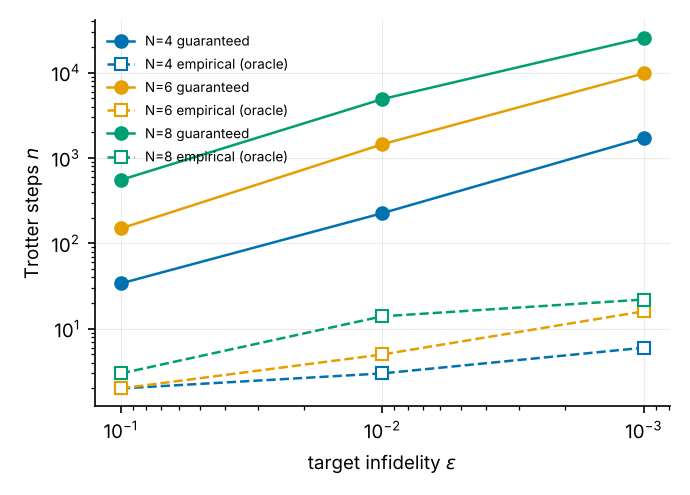
\includegraphics[width=0.7\textwidth,height=\textheight]{figs/fig1_guar_vs_emp.png}
\caption{Guaranteed (solid) and empirical (open markers) Trotter step
counts versus target infidelity.}
\end{figure}

\begin{longtable}[]{@{}
  >{\raggedright\arraybackslash}p{(\columnwidth - 20\tabcolsep) * \real{0.0909}}
  >{\raggedright\arraybackslash}p{(\columnwidth - 20\tabcolsep) * \real{0.0909}}
  >{\raggedright\arraybackslash}p{(\columnwidth - 20\tabcolsep) * \real{0.0909}}
  >{\raggedright\arraybackslash}p{(\columnwidth - 20\tabcolsep) * \real{0.0909}}
  >{\raggedright\arraybackslash}p{(\columnwidth - 20\tabcolsep) * \real{0.0909}}
  >{\raggedright\arraybackslash}p{(\columnwidth - 20\tabcolsep) * \real{0.0909}}
  >{\raggedright\arraybackslash}p{(\columnwidth - 20\tabcolsep) * \real{0.0909}}
  >{\raggedright\arraybackslash}p{(\columnwidth - 20\tabcolsep) * \real{0.0909}}
  >{\raggedright\arraybackslash}p{(\columnwidth - 20\tabcolsep) * \real{0.0909}}
  >{\raggedright\arraybackslash}p{(\columnwidth - 20\tabcolsep) * \real{0.0909}}
  >{\raggedright\arraybackslash}p{(\columnwidth - 20\tabcolsep) * \real{0.0909}}@{}}
\toprule\noalign{}
\begin{minipage}[b]{\linewidth}\raggedright
\(N\)
\end{minipage} & \begin{minipage}[b]{\linewidth}\raggedright
\(\varepsilon\)
\end{minipage} & \begin{minipage}[b]{\linewidth}\raggedright
\(n_{\mathrm{guar}}\)
\end{minipage} & \begin{minipage}[b]{\linewidth}\raggedright
\(n_{\mathrm{emp}}\)
\end{minipage} & \begin{minipage}[b]{\linewidth}\raggedright
ratio
\end{minipage} & \begin{minipage}[b]{\linewidth}\raggedright
bound \(1-F\)
\end{minipage} & \begin{minipage}[b]{\linewidth}\raggedright
measured \(1-F\) at \(n_{\mathrm{guar}}\)
\end{minipage} & \begin{minipage}[b]{\linewidth}\raggedright
sharpened bound
\end{minipage} & \begin{minipage}[b]{\linewidth}\raggedright
\(n_{\mathrm{guar}}^{\mathrm{sharp}}\)
\end{minipage} & \begin{minipage}[b]{\linewidth}\raggedright
CX guar.
\end{minipage} & \begin{minipage}[b]{\linewidth}\raggedright
CX emp.
\end{minipage} \\
\midrule\noalign{}
\endhead
\bottomrule\noalign{}
\endlastfoot
4 & \(10^{-1}\) & 34 & 2 & 17 & 0.0999 & 3.2e-3 & 0.035 & 14 & 723 &
51 \\
4 & \(10^{-2}\) & 226 & 3 & 75 & 0.0100 & 2.7e-4 & 3.2e-3 & 100 & 4 755
& 72 \\
4 & \(10^{-3}\) & 1 719 & 6 & 287 & 0.0010 & 3.1e-5 & 3.2e-4 & 760 & 36
108 & 135 \\
6 & \(10^{-1}\) & 150 & 2 & 75 & 0.0996 & 6.6e-3 & 0.034 & 60 & 5 265 &
85 \\
6 & \(10^{-2}\) & 1 450 & 5 & 290 & 0.0100 & 7.6e-4 & 3.5e-3 & 589 & 50
765 & 190 \\
6 & \(10^{-3}\) & 9 797 & 16 & 612 & 0.0010 & 2.8e-5 & 3.2e-4 & 4 328 &
342 910 & 575 \\
8 & \(10^{-1}\) & 555 & 3 & 185 & 0.0962 & 1.2e-2 & 0.038 & 175 & 27 216
& 168 \\
8 & \(10^{-2}\) & 4 903 & 14 & 350 & 0.0100 & 1.6e-4 & 3.2e-3 & 2 164 &
240 268 & 707 \\
8 & \(10^{-3}\) & 25 634 & 22 & 1 165 & 0.0010 & (not simulated) & -- &
11 317 & 1 256 087 & 1 099 \\
\end{longtable}

(\(J_2=0\), \(L=1\), floor design.
\(n_{\mathrm{guar}}^{\mathrm{sharp}}\) is the a-priori step number if
the sharpened composition of §3 replaced R4, computed on the un-gridded
design, i.e.~indicative.)

Three observations.

\emph{(a) The guarantee is sound but loose.} No design violated its
bound. The measured infidelity at \(n_{\mathrm{guar}}\) is 8--63× below
the bound, and the sharpened composition (valid in every case) tightens
the bound by 2.5--3.1× and reduces the a-priori \(n\) by 2.3--3.2×. Two
further sources of slack remain: the commutator norm is a worst case
over the full Hilbert space (the pulse-level operator error is already
only \(\le 0.24\) of the bound, §5.1) and the state error on low-energy
states is far smaller than the operator error (measured state error
\(2\times10^{-4}\) vs.~bound \(5.6\times10^{-2}\) at \(N=6\),
\(\varepsilon=10^{-2}\)).

\begin{figure}
\centering
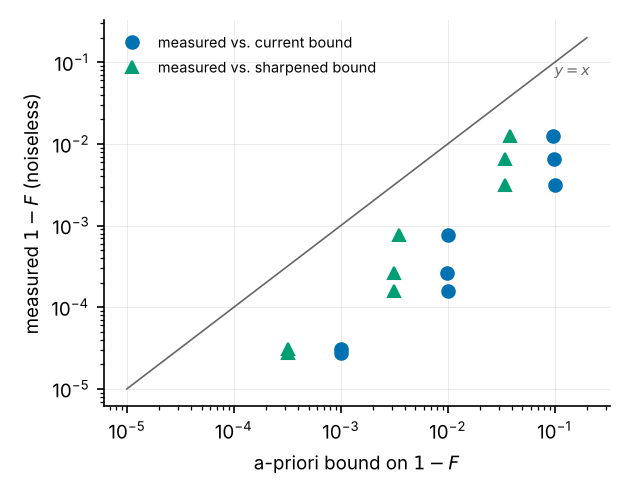
\includegraphics[width=0.55\textwidth,height=\textheight]{figs/fig2_bound_tightness.png}
\caption{Measured infidelity vs.~a-priori bound. All points lie below
\(y=x\).}
\end{figure}

\emph{(b) The ``empirical'' point is an oracle and sometimes not a
filter at all.} \(n_{\mathrm{emp}}\) is defined by comparison with the
exact ground state. In several rows (e.g.~\(N=6\),
\(\varepsilon=10^{-1},10^{-2}\); \(N=8\), \(\varepsilon=10^{-1}\)) the
certified \(\eta\) at \(n_{\mathrm{emp}}\) is \(\approx1\): the snapped
Trotter step (\(dt\approx3.6\) in scaled units, i.e.~\(W\,dt\approx13\)
rad) is so coarse that the circuit is no longer an approximation of the
designed filter, and the measured improvement is a property of that
particular discretisation, not something a bound can certify or a user
could know a priori. The empirical numbers should be presented as a
lower envelope, not as the algorithm's cost.

\emph{(c) Cost.} The guaranteed circuits for \(N=6\) at
\(\varepsilon=10^{-2}\) have 1450 Trotter steps, 50 765 CX, depth
\(\approx2\times10^{5}\) and \(\approx7\times10^{4}\) non-Clifford
rotations, i.e.~\(\sim1.4\times10^{6}\) T gates under the code's own
synthesis estimate, with success probability
\(P_{\mathrm{succ}}\approx0.72\).

\hypertarget{is-the-filter-worth-it-baselines}{%
\subsubsection{5.3 Is the filter worth it?
Baselines}\label{is-the-filter-worth-it-baselines}}

\begin{figure}
\centering
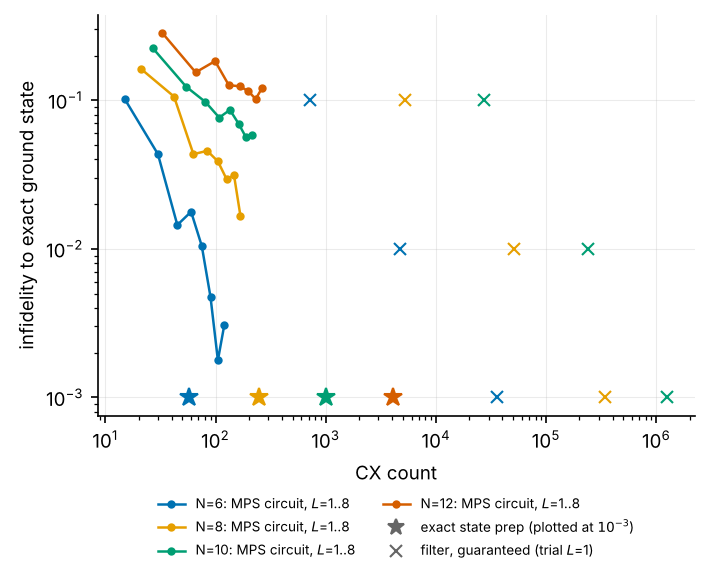
\includegraphics[width=0.7\textwidth,height=\textheight]{figs/fig3_baseline.png}
\caption{CX versus infidelity for the DMRG-derived MPS circuit
(\(L=1..8\)), exact state preparation (stars, plotted at a nominal
\(10^{-3}\)) and the guaranteed filter (crosses).}
\end{figure}

Exact preparation of the ED ground state with qiskit's generic isometry
synthesis costs 57, 247, 1013 and 4083 CX for \(N=6,8,10,12\)
(\(\approx2^{N}\)). The guaranteed filter at \(\varepsilon=10^{-2}\)
costs 50 765, 240 268 and 696 807 CX for \(N=6,8,10\),
i.e.~\textbf{890×, 970× and 690×} more than exact preparation, and 2--3
orders of magnitude more than the entire \(L\le8\) MPS-circuit family
(15--264 CX). The MPS-circuit baseline is itself imperfect and
\emph{non-monotone in \(L\)} (e.g.~\(N=6\): infidelity
\(1.4\times10^{-2}\) at \(L=3\), \(1.8\times10^{-2}\) at \(L=4\); the
compilation is a local optimisation), and at \(N=10,12\) it has not
converged by \(L=8\) (5.8 \% and 12 \% infidelity). Extrapolating the
fitted \(N^5\) filter cost against the \(2^N\) exact cost suggests a
crossover near \(N\approx26\) --- but dense isometry synthesis is not
available at that size and the extrapolation ignores the decay of
\(\gamma\) with \(N\); the relevant comparators there are MPS-based
sequential preparation {[}7{]} and QETU/Lin--Tong filters {[}5,6{]}.
\textbf{This comparison is the most important missing piece of the
present study.}

\hypertarget{scaling-with-system-size}{%
\subsubsection{5.4 Scaling with system
size}\label{scaling-with-system-size}}

\begin{figure}
\centering
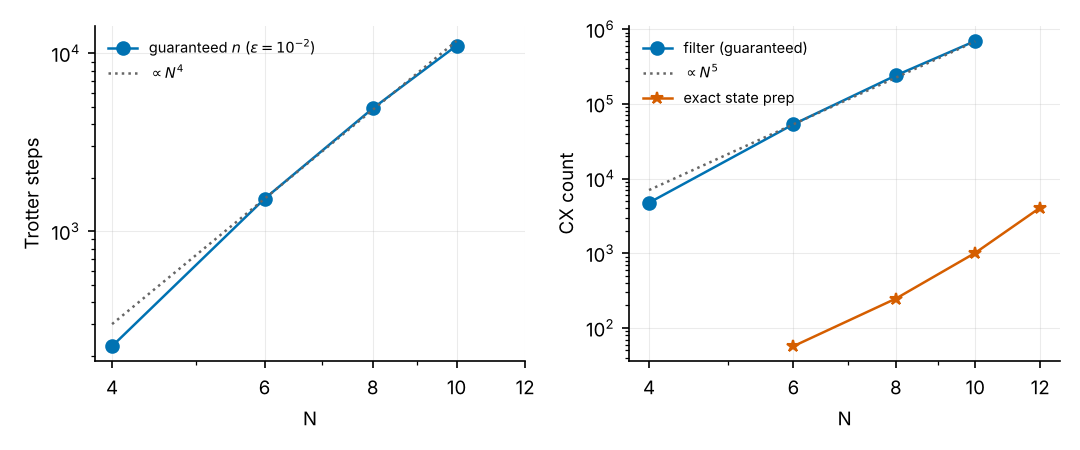
\includegraphics{figs/fig4_scaling.png}
\caption{Left: guaranteed Trotter steps at \(\varepsilon=10^{-2}\)
versus \(N\). Right: guaranteed CX versus \(N\), compared with exact
state preparation.}
\end{figure}

Guaranteed \(n\) for \(N=4,6,8,10\): 226, 1523, 4903, 11 060 (fit
exponent 4.3 over 4--10, 3.9 over 6--10); CX: \(4.8\times10^3\),
\(5.3\times10^4\), \(2.4\times10^5\), \(7.0\times10^5\) (exponent
5.0--5.5). This agrees with the structure of the bound,
\(n\propto\alpha_{\mathrm{phys}}T_{\mathrm{phys}}^{2}/(\sqrt{p_g}\,d_T)\)
with \(\alpha_{\mathrm{phys}}\propto N\) (3.0, 4.5, 6.0 for \(N=6,8,10\)
at \(J_2=0\)),
\(T_{\mathrm{phys}}\propto1/\Delta_{\mathrm{gap}}\propto N\) (gap 0.49,
0.39, 0.33) giving \(N^3\), with the remaining power from \(\gamma(N)\)
falling at fixed \(L\) (0.90, 0.84, 0.78) and hence tighter \(\eta_*\),
plus the per-step CX growing \(\propto N\). (Note that rescaling by
\(W\) cancels: \(\alpha T^2\) is \(W\)-independent.) Using \(L=3\) trial
layers raises \(\gamma\) (0.98, 0.94, 0.90 for \(N=6,8,10\)) and lowers
guaranteed CX by 3.2×, 1.7× and 1.5× respectively: the benefit of a
better trial state shrinks with \(N\) because the evolution time
\(T\propto1/\Delta_{\mathrm{gap}}\) is set by the gap, not by
\(\gamma\).

\hypertarget{the-dmrg-derived-inputs}{%
\subsubsection{5.5 The DMRG-derived
inputs}\label{the-dmrg-derived-inputs}}

\begin{longtable}[]{@{}
  >{\raggedright\arraybackslash}p{(\columnwidth - 12\tabcolsep) * \real{0.1429}}
  >{\raggedright\arraybackslash}p{(\columnwidth - 12\tabcolsep) * \real{0.1429}}
  >{\raggedright\arraybackslash}p{(\columnwidth - 12\tabcolsep) * \real{0.1429}}
  >{\raggedright\arraybackslash}p{(\columnwidth - 12\tabcolsep) * \real{0.1429}}
  >{\raggedright\arraybackslash}p{(\columnwidth - 12\tabcolsep) * \real{0.1429}}
  >{\raggedright\arraybackslash}p{(\columnwidth - 12\tabcolsep) * \real{0.1429}}
  >{\raggedright\arraybackslash}p{(\columnwidth - 12\tabcolsep) * \real{0.1429}}@{}}
\toprule\noalign{}
\begin{minipage}[b]{\linewidth}\raggedright
\(N\)
\end{minipage} & \begin{minipage}[b]{\linewidth}\raggedright
\(|\Delta E_0|\)
\end{minipage} & \begin{minipage}[b]{\linewidth}\raggedright
\(\Delta E_1=E_1^{\mathrm{DMRG}}-E_1\)
\end{minipage} & \begin{minipage}[b]{\linewidth}\raggedright
rel. gap error
\end{minipage} & \begin{minipage}[b]{\linewidth}\raggedright
\(|\Delta E_{\mathrm{top}}|\)
\end{minipage} & \begin{minipage}[b]{\linewidth}\raggedright
\(\mathrm{Var}(H)\)
\end{minipage} & \begin{minipage}[b]{\linewidth}\raggedright
\(|\langle\psi_{\mathrm{DMRG}}|E_0\rangle|^2\)
\end{minipage} \\
\midrule\noalign{}
\endhead
\bottomrule\noalign{}
\endlastfoot
6 & 3e-15 & −4e-16 & −7e-15 & 3e-15 & ≈0 & 1.0 \\
8 & 2e-15 & 2e-15 & 1e-15 & 5e-15 & ≈0 & 1.0 \\
10 & 5e-10 & 3.5e-10 & −3.7e-10 & 3e-13 & 2.5e-9 & 1.0 \\
12 & 1.2e-9 & 9.3e-10 & −8.5e-10 & 4e-12 & 5.8e-9 & 1.0 \\
14 & 1.8e-9 & 1.3e-9 & −2.0e-9 & 7e-12 & 8.3e-9 & 1.0 \\
16 & 2.2e-9 & 2.4e-9 & 7e-10 & 1e-11 & 1.0e-8 & 1.0 \\
\end{longtable}

(\(J_2=0\). Rows with ≈0 variance are at rounding level. \(J_2=0.2411\)
(\(N=6\)--\(16\)) and \(J_2=0.5\) (\(N=6\)--\(10\)) show the same
behaviour: \(|\Delta E_0|,|\Delta E_1|\le2.6\times10^{-9}\), overlap 1;
the full table is in \texttt{results/exp3a\_*.json}, which is written
when the sweep finishes.) DMRG reproduces \(E_0\), \(E_1\) and
\(E_{\mathrm{top}}\) to \(\lesssim2\times10^{-9}\) and the ground state
to overlap 1 against sparse-Lanczos ED up to \(N=16\). Three caveats are
relevant to certification, not to accuracy:

\begin{enumerate}
\def\labelenumi{\arabic{enumi}.}
\tightlist
\item
  \(\Delta E_1\ge0\) (up to rounding), as expected for a variational
  excited-state energy --- the \textbf{unsafe direction} for a gap used
  as a \emph{lower} bound. The size is negligible here, but nothing
  guarantees it for large \(N\) or frustrated \(J_2\).
\item
  The relative gap error changes sign, so the sign of the error is not
  controlled either.
\item
  The code's \(e_0=\sqrt{\mathrm{Var}H}/W\) (e.g.~\(10^{-4}/W\) at
  \(N=16\)) is five orders of magnitude larger than the true energy
  error (\(2\times10^{-9}\)): it is simultaneously non-rigorous (an
  eigenvalue within \(\sqrt{\mathrm{Var}}\) need not be the lowest) and
  wasteful (it enters \(|F(E_0)|\ge|F(0)|-Le_0\)). A Temple-type lower
  bound
  \(E_0\ge\langle H\rangle-\mathrm{Var}/(\tilde E_1-\langle H\rangle)\),
  which is \emph{quadratically} smaller, becomes available as soon as a
  rigorous lower bound \(\tilde E_1\) on the first excitation is
  accepted --- the same quantity the certificate already needs.
\end{enumerate}

(The DMRG penalty state \(\psi_1\) has weight 0.03--0.56 on any
\emph{single} ED vector at \(E_1\) because \(E_1\) is a
threefold-degenerate triplet; this is not an error.)

\hypertarget{over-estimating-the-gap-and-what-symmetry-could-buy}{%
\subsubsection{5.6 Over-estimating the gap, and what symmetry could
buy}\label{over-estimating-the-gap-and-what-symmetry-could-buy}}

We designed filters for a gap over-estimated by
\(s\in\{-20\%,\dots,+100\%\}\) (\(N=6\), \(J_2=0\),
\(\varepsilon_\ell=10^{-3}\)) and evaluated them on the true spectrum.

\begin{figure}
\centering
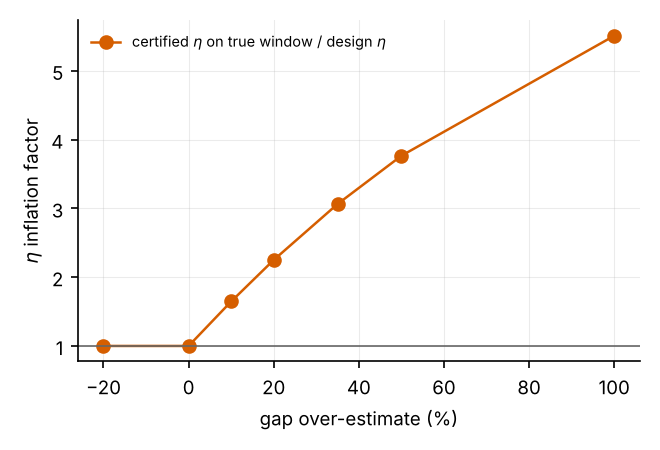
\includegraphics[width=0.55\textwidth,height=\textheight]{figs/fig5_gap_sensitivity.png}
\caption{Inflation of the certified \(\eta\) when the design gap exceeds
the true gap.}
\end{figure}

The certificate fails as soon as the design gap exceeds the true one:
certified \(\eta\) on the true window rises from 0.092 to 0.15, 0.21,
0.28, 0.34 and 0.50 for \(s=10,20,35,50,100\%\) (design target 0.092).
The \emph{measured} leakage of this particular trial state nevertheless
stays below the \(10^{-3}\) target (\(\le7\times10^{-4}\)). The reason
is symmetry: the \(L=1\) trial state has 96.3 \% of its weight in
\(S=0\), 0.49 \% in \(S=1\), 3.2 \% in \(S=2\), and the triplet that
fixes the gap carries almost none of it, while the first \(S=0\)
excitation lies at 2.66× the triplet gap (\(N=6\), \(J_2=0\)). A
rigorous statement therefore needs the sector weights, which suggests a
concrete improvement (§6): because every bond exponential is
SU(2)-symmetric (``bond'' ordering) the Trotterised evolution preserves
\(S\), so one may certify with sector-dependent windows. The potential
saving, since \(n\propto\Delta^{-2}\), is
\((\Delta_{\mathrm{sector}}/\Delta_{\mathrm{any}})^2\):

\begin{longtable}[]{@{}llll@{}}
\toprule\noalign{}
\(J_2\) & \(N=6\) & \(N=8\) & \(N=10\) \\
\midrule\noalign{}
\endhead
\bottomrule\noalign{}
\endlastfoot
0 & 7.1× & 7.0× & 6.9× \\
0.2411 & 4.2× & 4.1× & 4.1× \\
0.5 & 1.8× & 1.6× & 1.4× \\
\end{longtable}

(ratio \((\Delta_{\mathrm{sector}}/\Delta_{\mathrm{any}})^2\) from exact
diagonalisation; \(N=12\), \(J_2=0\): 6.8×.)

\hypertarget{the-j_20.5-case-is-trivial-and-exposes-a-defect}{%
\subsubsection{\texorpdfstring{5.7 The \(J_2=0.5\) case is trivial, and
exposes a
defect}{5.7 The J\_2=0.5 case is trivial, and exposes a defect}}\label{the-j_20.5-case-is-trivial-and-exposes-a-defect}}

At the Majumdar--Ghosh point the open even chain has the
product-of-dimers ground state {[}8{]}, which a single brickwork layer
reproduces exactly: we find \(\gamma=1\) (to double precision) for
\(N=4\)--\(12\). \texttt{floor\_vs\_precision} then correctly returns
``no filter needed'' rows (\(m=0\)), but \texttt{choose\_floor\_design}
counts them as infeasible and \texttt{make\_design} silently falls back
to the legacy \texttt{builder} design with a hard-coded
\(P_{\mathrm{succ}}\ge0.9\). The pipeline then reports guaranteed
circuits of 24 261, 511 068 and 1 157 409 CX for \(N=4,8,10\) to prepare
a state it already has, and the oracle-empirical search ``meets''
\(\varepsilon=0.1\) with a state that has \emph{lost} 9 \% fidelity. The
near-MG regime is therefore a poor benchmark for the algorithm; the
interesting frustrated regime is \(J_2\sim0.3\)--\(0.45\) or
non-dimerised trial limits (small \(L\) at larger \(N\)). \#\# 6. Code
audit and recommended changes

Severity: \textbf{H} invalidates a claim or can silently produce a
wrong/ruinous result; \textbf{M} weakens a claim or wastes resources;
\textbf{L} hygiene. Line references are to \texttt{AARON/j1j2\_filter}.

\begin{longtable}[]{@{}
  >{\raggedright\arraybackslash}p{(\columnwidth - 8\tabcolsep) * \real{0.2000}}
  >{\raggedright\arraybackslash}p{(\columnwidth - 8\tabcolsep) * \real{0.2000}}
  >{\raggedright\arraybackslash}p{(\columnwidth - 8\tabcolsep) * \real{0.2000}}
  >{\raggedright\arraybackslash}p{(\columnwidth - 8\tabcolsep) * \real{0.2000}}
  >{\raggedright\arraybackslash}p{(\columnwidth - 8\tabcolsep) * \real{0.2000}}@{}}
\toprule\noalign{}
\begin{minipage}[b]{\linewidth}\raggedright
\#
\end{minipage} & \begin{minipage}[b]{\linewidth}\raggedright
Sev
\end{minipage} & \begin{minipage}[b]{\linewidth}\raggedright
Location
\end{minipage} & \begin{minipage}[b]{\linewidth}\raggedright
Finding
\end{minipage} & \begin{minipage}[b]{\linewidth}\raggedright
Recommended fix
\end{minipage} \\
\midrule\noalign{}
\endhead
\bottomrule\noalign{}
\endlastfoot
1 & H & \texttt{pipeline.choose\_floor\_design}, \texttt{make\_design} &
\(\gamma\ge1-\epsilon_{\mathrm{mach}}\) produces \(m=0\) rows that are
counted infeasible; fallback to \texttt{builder} (hard-coded
\(P_{\mathrm{succ}}\ge0.9\), no \(\eta\) target) builds a filter for an
already-exact state (24 k--1.2 M CX at \(J_2=0.5\), §5.7). Mixed
\texttt{floor}/\texttt{builder} rows are also not comparable. & Return
the identity (``no filter, cost 0'') when \(\gamma\) is within tolerance
of 1, and never mix design sources in one table. \\
2 & H & \texttt{core/spectrum.get\_spectrum} (DMRG path),
\texttt{pipeline.build\_ctx} & Certificates are rigorous only if (A1)
\(\Delta\le\Delta_{\mathrm{true}}\), (A2)
\(\gamma\le\gamma_{\mathrm{true}}\), (A3)
\(|E_0^{\mathrm{shift}}-E_0|\le e_0\) hold; DMRG supplies none of them
(§4.1, §5.5--5.6). In the default ED mode the certified results are
limited to \(N\le12\). & State the theorem \emph{conditional on}
(A1)--(A3) with these labels; report \(\Delta\) with an explicit safety
margin; for large \(N\) obtain a gap lower bound by an independent
method (e.g.~symmetry-resolved DMRG plus a Temple/Weinstein-type bound)
or present the large-\(N\) numbers as estimates. \\
3 & H & \texttt{pipeline.ORDER}, \texttt{core/trotter.trotter\_bounds} &
The bound is first-order; setting \texttt{ORDER=2} changes the circuits
but the same \(\alpha t^2/2k\) bound is still reported (and
\texttt{lie\_trotter\_order} only checks order 1). &
\texttt{assert\ ORDER\ ==\ 1} next to the bound, or implement the
second-order commutator bound. \\
4 & H & \texttt{pipeline.build\_ctx}
(\texttt{if\ N\ \textless{}=\ 16:\ ...\ eigvalsh(Hs.toarray())}) & Dense
\(2^N\times2^N\) complex matrix: 4.3 GB at \(N=14\), 68.7 GB at
\(N=16\); \texttt{SOURCE=\textquotesingle{}dmrg\textquotesingle{}} is
advertised for \(N>12\). & Cap the dense check at \(N\le12\) or use
\texttt{eigsh} for the two extremal eigenvalues. \\
5 & H & repo & Not reproducible as shipped:
\texttt{scripts/run\_study.py} imports a \texttt{study} module that is
absent; \texttt{mps\_to\_circuit} is an unpinned external dependency
that fails on Python ≥ 3.13; \texttt{main.ipynb} imports a stale
831-line monolith \texttt{builder.py}, and
\texttt{hamiltonians.py}/\texttt{get\_energies.py} exist twice; comments
cite tests (``T1'', ``T8'', audit items A1--A14) that are not in the
repository. & Add \texttt{study.py}, a pinned
\texttt{requirements.txt}/lock file, delete or archive
\texttt{builder.py}, single-source the two duplicated modules, and add a
\texttt{tests/} directory containing the checks of §5.1 (our
\texttt{exp1\_primitives.py} can be the seed). \\
6 & M & \texttt{floor.floor\_vs\_precision}
vs.~\texttt{pipeline.choose\_floor\_design} & The \((x,m)\) winner for
each \(\varepsilon\) is picked with proxy \(x^2/F(0)^2\), but the true
cost is \(n/P\propto x^2/F(0)^{3}\) (since \(n\propto1/\sqrt{p_g}\));
the later choice over leakage fractions uses the correct cost, so the
two stages optimise different objectives. & Pass
\texttt{cost\_fn=lambda\ x,f,m:\ x*x/f**1.5}. \\
7 & M & \texttt{pipeline.find\_empirical} & ``Empirical'' \(n\) uses the
exact ground state and can land where \(\eta\approx1\) (§5.2b). & Report
it only as an oracle lower envelope; require certified \(\eta<1\). \\
8 & M & \texttt{pipeline.costs} & Expected cost
\(=\mathrm{CX}_{\mathrm{total}}/P_{\mathrm{succ}}\) ignores early abort
(a failed pulse stops the run), so it overestimates; correct form:
\(\bigl(c_{\mathrm{trial}}+\sum_i c_{\mathrm{step}}k_i\prod_{j<i}p_j\bigr)/\prod_jp_j\).
& Implement with the per-pulse \(p_j\) that the simulation already
has. \\
9 & M & \texttt{pipeline} (\texttt{hi=1.0} everywhere);
\texttt{core/spectrum} & The filter must suppress \([\Delta,1]\), but
the spectrum ends at \((E_{\mathrm{top}}-E_0)/W<1\) when \(W\) is the
certified (looser) bandwidth; \(W=c_I+\sum|c_\beta|-E_0\) overstates
\(E_{\mathrm{top}}\) by 3× because \(XX{+}YY{+}ZZ\) is bounded termwise
(true per-bond bound \(J/4\), so
\(E_{\mathrm{top}}\le\frac14[J_1(N-1)+J_2(N-2)]\) for \(J\ge0\)). & Pass
\texttt{hi=(E\_top\_bound-E0)/W} and use the per-bond bound, which is
also rigorous and 3× tighter. \\
10 & M & \texttt{core/trotter.total\_error\_bound} & Composition
\((\sqrt{2\ell}+d_T)^2\) with \(d_T=2\epsilon_T/\sqrt{p_g}\) is valid
but 2.5--3.1× loose. & Use
\(\sin^2(\arcsin\sqrt\ell+\arcsin(\epsilon_T/\sqrt{p_g}))\)
(Proposition, §3; verified in all simulated cases). \\
11 & M & \texttt{core/\_\_init\_\_},
\texttt{core/resources.rotation\_synthesis\_t\_count} & The authors
themselves flag the Trotter theorem statement and the synthesis
constants (\(1.15\log_2(1/\epsilon)+9.2\)) as ``quoted from memory''. &
Verify against the sources and cite them in the paper before reporting
T-counts. \\
12 & L & \texttt{core/circuits.h\_tensor\_z} & The shift term
\(-E_0/W\cdot Z_{\mathrm{anc}}\) is applied as a separate non-Clifford
\(R_z\) in every Trotter step; it commutes with everything and can be
folded into \(\phi_i\) (\(\phi_i\to\phi_i-E_0t_i/W\)), saving one of 47
non-Clifford rotations per step (\(N=6\)). & Fold into the phase. \\
13 & L & \texttt{pipeline.build\_ctx} & \(\gamma\) is clipped with
\texttt{min(·,1)} but the \(\gamma=1\) branch is never propagated (see
1); the ED-vs-DMRG \(\gamma\) fallback is labelled but not carried into
reports. & Carry \texttt{gamma\_src} into every exported number. \\
\end{longtable}

\hypertarget{methodological-improvements-that-follow-from-the-analysis}{%
\subsubsection{6.1 Methodological improvements that follow from the
analysis}\label{methodological-improvements-that-follow-from-the-analysis}}

\begin{enumerate}
\def\labelenumi{\arabic{enumi}.}
\tightlist
\item
  \textbf{Sharpened composition} (item 10): a free, proven 2.5--3.1×
  tighter bound and 2.3--3.2× fewer guaranteed steps.
\item
  \textbf{Symmetry-resolved certification}: let \(w_s\) be the trial
  weight in sector \(s\) and \(\Delta_s\) the gap of that sector. Then
  \(\ell\le\sum_sw_s\,(\sup_{[\Delta_s,1]}|F|)^2/F(0)^2\) over the
  ground-state sector and the (small) remainder bounded with the global
  gap. Because bond-ordered Trotter steps are exactly SU(2)-symmetric,
  the sector weights are conserved by the (Trotterised) evolution, so
  this is rigorous given the sector weights, which are cheap to compute
  from the trial MPS. Potential saving up to
  \((\Delta_s/\Delta)^2\approx7\times\) in \(n\) at \(J_2=0\) (§5.6).
\item
  \textbf{Subspace-restricted Trotter bounds}: replace the global
  \(\alpha\) by commutator norms restricted to the low-energy subspace
  populated by the trial state (the observed state error is ≈ 300× below
  the bound), or use higher-order formulas with the matching commutator
  bound.
\item
  \textbf{Tensor-network simulation of the filter.} The DMRG advantage
  is lost as long as every number comes from dense vectors; the
  controlled evolution \(e^{-itH\otimes Z}\) is an MPO-friendly
  operation, so MPS/TEBD simulation of the Trotterised filter would
  allow \(N\sim30\)--\(100\) and show the real DMRG→circuit→filter
  story.
\end{enumerate}

\hypertarget{conclusions-and-what-a-publishable-paper-still-needs}{%
\subsection{7. Conclusions and what a publishable paper still
needs}\label{conclusions-and-what-a-publishable-paper-still-needs}}

\textbf{Established.} The mathematics of the filter, leakage, Trotter
and composition bounds is correct, and verified numerically in every
test performed; the pipeline's reference implementation (pulse
convention, MPO/Pauli agreement, circuit-vs-numpy agreement to
\(10^{-16}\)) is consistent; DMRG supplies ground-state and excitation
energies to \(\sim10^{-9}\) up to \(N=16\).

\textbf{Not established.} (i) A resource advantage: at \(N\le12\) the
guaranteed filter costs \(10^{2}\)--\(10^{3}\times\) exact preparation
and \(\gg\) shallow MPS circuits, and the empirical savings come from an
oracle. (ii) A DMRG-specific role in certification: the certified
numbers are ED-based. (iii) Anything at \(N>12\), near criticality or in
the frustrated regime away from the exactly solvable MG point.

\textbf{Required for submission (in priority order).}

\begin{enumerate}
\def\labelenumi{\arabic{enumi}.}
\tightlist
\item
  \emph{Baselines.} Compare resources at equal fidelity against (a)
  deeper/optimised MPS circuits and sequential MPS preparation, (b)
  QETU/Lin--Tong filtering with the same trial state, (c) rodeo with
  random times. Without this the paper cannot claim usefulness.
\item
  \emph{Large-\(N\) data} from a tensor-network simulation of the filter
  (item 4 above), with \(\gamma(N,L)\) and the gap from DMRG labelled as
  estimates, and a stated rigorous or heuristic gap input.
\item
  \emph{Tighter guarantees}: items 10 and 2 of §6.1 at minimum, to close
  the 100--1000× gap to the empirical cost, and an honest empirical
  definition (certified \(\eta<1\)).
\item
  \emph{Benchmarks that stress the algorithm}: \(J_2\in[0.2,0.45]\),
  \(N\ge16\), and trial states with \(\gamma\ll1\); drop \(J_2=0.5\) or
  use it only as a sanity check.
\item
  \emph{Repository hygiene} (items 1--5 of §6), a test suite, pinned
  environment, and archived raw data for every table and figure.
\item
  \emph{Resource model}: Hamiltonian-aware compilation of
  \(e^{-it\,h_b\otimes Z}\) (bond exponentials are SU(2)-symmetric),
  verified T-count constants, and a fault-tolerant estimate with
  early-abort statistics.
\end{enumerate}

\textbf{Suggested framing if the above is only partially achievable:} a
methods paper on \emph{certified} SBC filtering --- rigorous a-priori
bounds, symmetry-resolved certification, and a verification harness ---
rather than a performance paper.

\hypertarget{reproducibility}{%
\subsection{8. Reproducibility}\label{reproducibility}}

Code: \texttt{AARON/evaluation/experiments}
(\texttt{exp1\_primitives.py} building-block tests;
\texttt{exp2\_end\_to\_end.py\ N\ J2\ L};
\texttt{exp3\_dmrg\_inputs.py}; \texttt{exp3b\_baseline.py};
\texttt{exp4\_gap\_and\_symmetry.py}; \texttt{exp5\_scaling.py};
\texttt{make\_figures.py}). Raw outputs:
\texttt{AARON/evaluation/results/*.json}; logs:
\texttt{AARON/evaluation/logs}. All experiments call
\texttt{AARON/j1j2\_filter} unmodified. Environment: Python 3.12, numpy
2.x, scipy 1.18, qiskit 2.5.2, quimb 1.15, \texttt{mps-to-circuit}; run
with \texttt{OMP\_NUM\_THREADS=1} (multi-threaded BLAS made the SLSQP
filter design several times slower). Floor-design settings for the
scaling study were reduced for speed
(\texttt{FLOOR\_EPS\_FRACS={[}0.2,0.1,0.05{]}},
\texttt{FLOOR\_M={[}4,6{]}}); end-to-end runs used the defaults.

\textbf{Limitations of this evaluation.} Single trial-circuit
compilation per \((N,J_2,L)\) (the compiler is a local optimiser, so
\(\gamma\) is not unique); \(J_2\neq0,0.5\) end-to-end runs and \(N>10\)
end-to-end runs were not completed; the \(N=8\), \(\varepsilon=10^{-3}\)
guaranteed design was not simulated (beyond the simulation cap); the
scaling fits use four sizes; the crossover estimate is an extrapolation.
References were written from memory and must be checked before
submission.

\hypertarget{references}{%
\subsection{References}\label{references}}

\begin{enumerate}
\def\labelenumi{\arabic{enumi}.}
\tightlist
\item
  I. Stetcu, A. Baroni, J. Carlson, \emph{Projection algorithm for state
  preparation on quantum computers}, Phys. Rev.~C \textbf{105}, 064308
  (2022).
\item
  K. Choi, D. Lee, J. Bonitati, Z. Qian, J. Watkins, \emph{Rodeo
  algorithm for quantum computing}, Phys. Rev.~Lett. \textbf{127},
  040505 (2021).
\item
  Z. Qian et al., \emph{Demonstration of the rodeo algorithm on a
  quantum computer}, arXiv:2110.07747.
\item
  A. M. Childs, Y. Su, M. C. Tran, N. Wiebe, S. Zhu, \emph{Theory of
  Trotter error with commutator scaling}, Phys. Rev.~X \textbf{11},
  011020 (2021).
\item
  L. Lin, Y. Tong, \emph{Near-optimal ground state preparation}, Quantum
  \textbf{4}, 372 (2020).
\item
  Y. Dong, L. Lin, Y. Tong, \emph{Ground-state preparation and energy
  estimation on early fault-tolerant quantum computers via quantum
  eigenvalue transformation of unitary matrices}, PRX Quantum
  \textbf{3}, 040305 (2022).
\item
  C. Schön, E. Solano, F. Verstraete, J. I. Cirac, M. M. Wolf,
  \emph{Sequential generation of entangled multiqubit states}, Phys.
  Rev.~Lett. \textbf{95}, 110503 (2005).
\item
  C. K. Majumdar, D. K. Ghosh, \emph{On next-nearest-neighbor
  interaction in linear chain}, J. Math. Phys. \textbf{10}, 1388 (1969).
\item
  S. R. White, \emph{Density matrix formulation for quantum
  renormalization groups}, Phys. Rev.~Lett. \textbf{69}, 2863 (1992); U.
  Schollwöck, Ann. Phys. \textbf{326}, 96 (2011).
\item
  K. Okamoto, K. Nomura, Phys. Lett. A \textbf{169}, 433 (1992).
\end{enumerate}

\end{document}
